\documentclass[a4paper]{article}

\usepackage{graphicx}
\usepackage{amsmath,amssymb}
\usepackage{minted}
\usepackage{multirow}
\usepackage{float}
\usepackage{algorithm}
\usepackage{algpseudocode}
\usepackage{todonotes}
\usepackage{forest}
\usepackage{xstring}
\usepackage{xcolor}
\usepackage[most]{tcolorbox}
\usepackage{xparse}
\usepackage{natbib}
\usepackage{adjustbox}

\usetikzlibrary{graphs,graphdrawing}
\usegdlibrary{layered}

% for external graphviz
\input{/home/donkarlo/Dropbox/repo/nd_language_ai_project/src/nd_language_ai/formal/computer/programming/tex/latex/code_clips/external_graphviz.tex}

% for tags
\input{/home/donkarlo/Dropbox/repo/nd_language_ai_project/src/nd_language_ai/formal/computer/programming/tex/latex/part/control_sequence/kind/semtag/semtag.tex}

% for links
\input{/home/donkarlo/Dropbox/repo/nd_language_ai_project/src/nd_language_ai/formal/computer/programming/tex/latex/code_clips/seehere.tex}

% for nested lists and sections
\input{/home/donkarlo/Dropbox/repo/nd_language_ai_project/src/nd_language_ai/formal/computer/programming/tex/latex/code_clips/deep_structure.tex}

\title{}
\date{}
\author{Mohammad Rahmani}

\begin{document}
   \maketitle

   On one side of the square corridor, the corridor becomes symmetrically narrower,\ref{} and consequently the human controller sends necessary commands to uav1
   \begin{figure}[H]
      \centering
      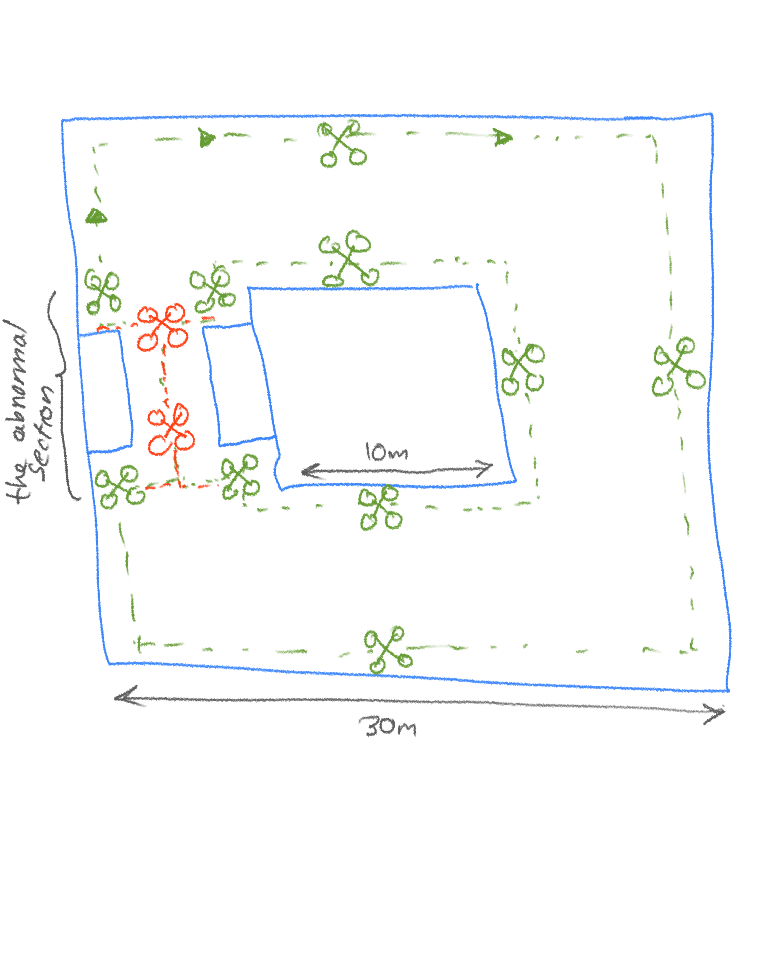
\includegraphics[width=0.9\textwidth]{follow_scenario_specification.png}
   \end{figure}

   \begin{figure}[H]
      \centering
      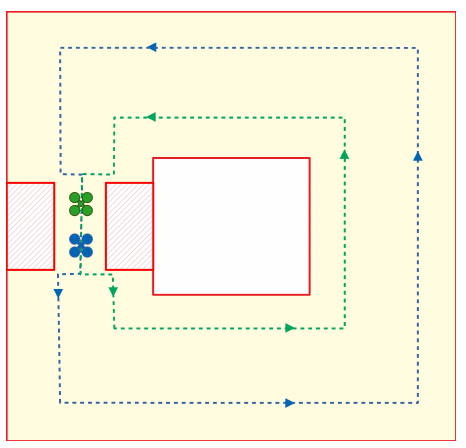
\includegraphics[width=0.5\textwidth]{follow.png}
      \label{follow}
   \end{figure}
   \section{Anomaly results}
   IN different runs results might vary
      \begin{figure}[H]
         \centering
         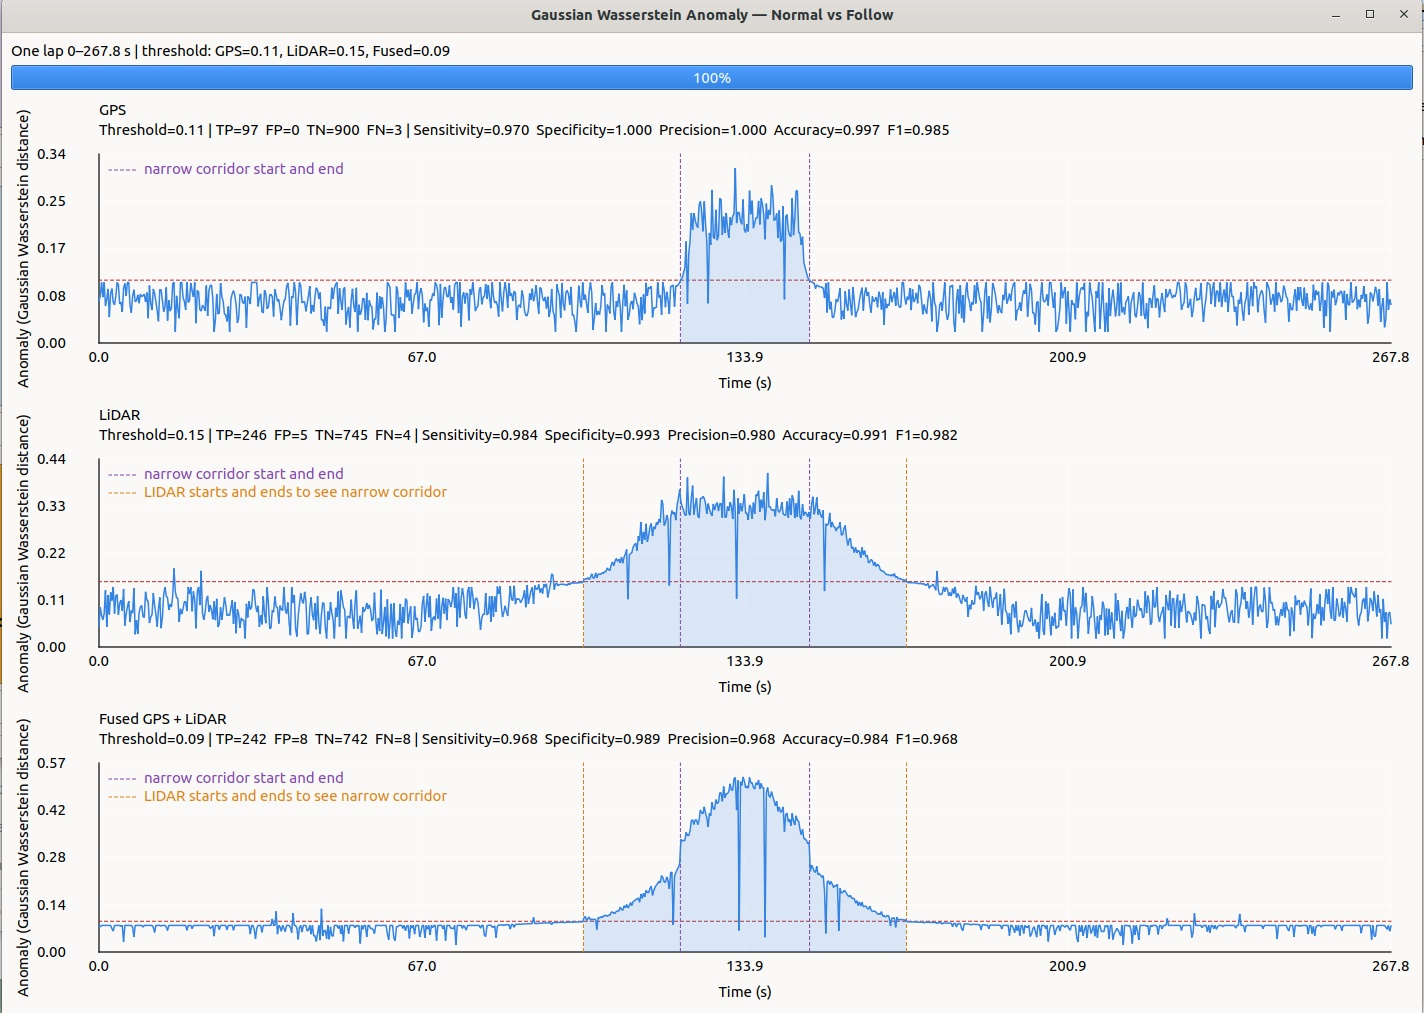
\includegraphics[width=0.9\textwidth]{anomaly_signals.jpg}
      \end{figure}

   \section{Results}

      \begin{table}[H]
         \centering
         \caption{GPS anomaly detection results.}
         \begin{tabular}{lc}
            \hline
            Metric & Value \\
            \hline
            Threshold & 0.11 \\
            True Positive (TP) & 97 \\
            False Positive (FP) & 0 \\
            True Negative (TN) & 900 \\
            False Negative (FN) & 3 \\
            Sensitivity & 0.970 \\
            Specificity & 1.000 \\
            Precision & 1.000 \\
            Accuracy & 0.997 \\
            F1-score & 0.985 \\
            \hline
         \end{tabular}
      \end{table}

      \begin{table}[H]
         \centering
         \caption{LiDAR anomaly detection results.}
         \begin{tabular}{lc}
            \hline
            Metric & Value \\
            \hline
            Threshold & 0.15 \\
            True Positive (TP) & 246 \\
            False Positive (FP) & 5 \\
            True Negative (TN) & 745 \\
            False Negative (FN) & 4 \\
            Sensitivity & 0.984 \\
            Specificity & 0.993 \\
            Precision & 0.980 \\
            Accuracy & 0.991 \\
            F1-score & 0.982 \\
            \hline
         \end{tabular}
      \end{table}

      \begin{table}[H]
         \centering
         \caption{Fused GPS and LiDAR anomaly detection results.}
         \begin{tabular}{lc}
            \hline
            Metric & Value \\
            \hline
            Threshold & 0.09 \\
            True Positive (TP) & 242 \\
            False Positive (FP) & 8 \\
            True Negative (TN) & 742 \\
            False Negative (FN) & 8 \\
            Sensitivity & 0.968 \\
            Specificity & 0.989 \\
            Precision & 0.968 \\
            Accuracy & 0.984 \\
            F1-score & 0.968 \\
            \hline
         \end{tabular}
      \end{table}
      \bibliographystyle{plainnat}
      \bibliography{/home/donkarlo/Dropbox/repo/nd_shared_research/bibliography/bibliography.bib}
\end{document}
